\chapter{Methodology}
%%%%%%%%%%
This chapter outlines the underlying methodology of this work. Following \cite{gilljohnson}, the sequence of a research process is identify area (1), select research topic (2), decide on approach (3), formulate plan (4), collect data (5),  analyze data (6), present findings (7). With the first two steps being motivated and further specified in \ref{chap:case}, this section especially reasons approach (3), plan (4) and data aspects (5). 

This thesis is part of a wider research project targeting processes, data and analytics in omni-channel CRM. The methodology described in the following refers to this thesis only and not to the superordinate research project. Prior work in the project helped to create a foundation where this work can build on. \acrfull{DSR} is chosen as the research design, which is described in detail in the following sections, along with the epistemological aspects. Data was gathered in interviews with domain experts, supported by literature, as well as documents from the research partner. Descriptions of these data sources complete this chapter. 


	\section{Epistemological Perspective}
	\label{sec:epis}
	%%%%%%%%%%		
Stating the epistemological view of this work helps to support the reader in understanding the author's statements. Furthermore, it demonstrates a systematical method, which is sometimes perceived as lacking in qualitative research. Drawing on a framework by \cite{becker2007epistemological}, five questions are mentioned in order to structure the epistemological positioning of research. The concepts highlighted in bold represent the approach taken in this thesis. 

\begin{enumerate}
	\item What is the object of cognition? (Ontological aspect)
		\subitem \textbf{Ontological Realism} | Ontological idealism  | Kantianism
	\item What is the relationship between cognition and the object of cognition?
		\subitem Epistemological realism | \textbf{Constructivism}
	\item What is true cognition? (Concept of truth)
		\subitem Correspondence |  \textbf{Consensus} |  Semantic theory of truth
	\item Where does cognition originate?
	\subitem Empiricism | Rationalism | \textbf{Kantianism}
	\item By what means can cognition be achieved? (Methodological aspect)
		\subitem \textbf{Inductivism} | \textbf{Deductivism} | \textbf{Hermeneutic}
\end{enumerate}

%\begin{table}[caption={Epistemological perspective}, label=fig:epi]
%	\centering
%	\begin{tabular}{|p{6cm}|p{1.5cm}|p{1.5cm}|p{1.5cm}|p{1.5cm}|p{1.5cm}|p{1.5cm}|}
%		\hline
%		\textit{What is the object of cognition? (Ontological aspect)}                   & \multicolumn{2}{l|}{\textbf{Ontological Realism}} & \multicolumn{2}{l|}{Ontological idealism} & \multicolumn{2}{l|}{Kantianism}               \\ \hline
%		\textit{What is the relationship between cognition and the object of cognition?} & \multicolumn{3}{l|}{Epistemological realism}                            & \multicolumn{3}{l|}{\textbf{Constructivism}}                        \\ \hline
%		\textit{What is true cognition? (Concept of truth)}                              & \multicolumn{2}{l|}{Correspondence}               & \multicolumn{2}{l|}{\textbf{Consensus}}   & \multicolumn{2}{l|}{Semantic theory of truth} \\ \hline
%		\textit{Where does cognition originate?}                                         & \multicolumn{2}{l|}{Empiricism}                   & \multicolumn{2}{l|}{Rationalism}          & \multicolumn{2}{l|}{\textbf{Kantianism}}      \\ \hline
%		\textit{By what means can cognition be achieved? (Methodological aspect)}        & \multicolumn{2}{l|}{\textbf{Inductivism}}         & \multicolumn{2}{l|}{\textbf{Deductivism}} & \multicolumn{2}{l|}{\textbf{Hermeneutic}}     \\ \hline
%	\end{tabular}
%
%\end{table}

\subsubsection{Ad 1. Object of cognition}
Ontology is the science of \textit{what is} and \textit{how it is}. The existence and nature of reality are subject matter. Ontological realism assumes a real world that exists independently of cognition. Ontological idealism sees reality as a construct depending on human consciousness. Kantianism brings together the two mentioned views by distinguishing in the unknowable \enquote{thing-in-itself} and the appearing of those things to an observer. 

This work takes the view of ontological realism, as the construction of the reference model is intended to solve a real-world problem. Hence, this world should exist for every observer. 

\subsubsection{Ad 2. Relationship between cognition and the object of cognition}
This question asks whether entities beyond human thought can be recognized as objective (in principle). Epistemological realism affirms this question. Constructivism deems cognition as subjective and hence makes understanding a private construct determined by the subject. 

Because subjects that turn the reference model to account will show different understandings and requirements, the constructivistic view is taken. These subjects can be classified into reference model users and designers, that will see it from different angles from a group perspective, \eg scientific and practical. Moreover, every subject will interpret the model in a subjective manner.

\subsubsection{Ad 3. Concept of truth}
The \textit{true} cognition and how humans can achieve it is foci of this question and there are three theories \citep{habermas1973}. Correspondence theory of truth states that true statements refer to facts of the real world. This requires a realistic view in both ontology and epistemology. Consensus theory of truth bases on constructivism: A statement is true\textit{ for a group}, only if all peers agree and true if everyone agrees. Hence there can be no proof of truth. Thirdly, semantic theory of truth proposes that truth is always related to an object language where the possibly true statements are communicated in. Therefore there has to be a meta-language that is able to analyze the correctness of a statement in object language \citep{tarski1944}. 

Following the constructivistic view, the consensus theory of truth is selected. The correctness of modeling is dependent on the group of reference model users and its designers. If they find a consensus, truth can be achieved within the group. Application of the reference model changes the user group and implies changes in the model, so that it matches the circumstances in the company. The application model designers and users then again need to find a consensus.

\subsubsection{Ad 4. Origin of cognition}
There are three origins of cognition. Cognition from experience falls under the school of empiricism. Rationalism puts intellect as the source of cognition. Kantianism again combines both views so that both experience and intellect can be origin of cognition. 

Both intellect and experience are seen as integral parts of cognition in research. Cognitive efforts and reflections of the author are part of the reference model design. Practical experience, as included by the interview component, is used for evaluating the artifact. This requires avoiding direct use of interview content in artifact design, so that a self-fulfilling prophecy is prevented. 

\subsubsection{Ad 5. Methodological aspect}
While inductivism describes the extension from individual cases to universal laws, deductivism is the derivation of the individual from the universal \citep{seiffert2006einfhrung}. Hermeneutic assumes prior knowledge in an issue by a subject that is able to improve its understanding of \textit{the entire} by consumption of new knowledge. This repeating consumption shapes understanding and is called the hermeneutic cycle \citep{Butler1998}.

Inductivism is focal in reference modeling, as the case needs to be abstracted to achieve the required universality in reference modeling. Deductivism is also part, as general process  structures were applied to the domain of BPO and more specifically BPO in CRM. Both are common in construction of reference models \citep{thomas2006mang,Fettke2014meth}.

The act of design within this work is characterized by a hermeneutic aspect. The model is shaped by the consumption of existing scientific concepts, as well as requirements from the practical case. As the approach was to increase modeling detail over time, a repeating process emerged: First interviews derived high-level requirements, while the following gave new input that related to additional knowledge. This additional knowledge closes the circle as it became preknowledge to the next repetition. 

%%%%%%%%%%
\section{Design Science}
Research has to employ accepted methodologies to be accepted in the community. \citeauthor{creswell2013research} names the selection of a research approach as the first of preliminary considerations \citep{creswell2013research}. \acrfull{DSR}, as conceptualized by \cite{simon1996sciences} is getting more and more attention in the \acrshort{IS} field and will be the guiding paradigm for this thesis. 

Motivating this choice is \acrshort{DSR}'s overall goal to create innovative artifacts to solve real-world problems. This addresses the often criticized limited practical relevance in \acrshort{IS} research \citep{hirschheim}, while still employing the relevant rigor that separates it as a research project from the practice of routine design \citep{Winter2008Hevner}. Routine design, in contrast to \acrshort{DSR}, does not contribute to the knowledge base. The common understanding of \acrshort{DSR} today is based on in the work of \cite{Hevner2004}. It stands for a problem-\textit{solving} paradigm in contrast to behavioural science research, which takes a problem \textit{understanding} approach by developing theories. However, their complementary nature justifies both paradigms, as IS artifacts (as an outcome of \acrshort{DSR}) provide \textit{utility} and are subject to behavioral science research, which in turn provides \textit{truth} in form of theories to be used in \acrshort{DSR}.

			
\begin{figure}[caption={Design Science Research Cycles}, label={fig:dsr}]
	{	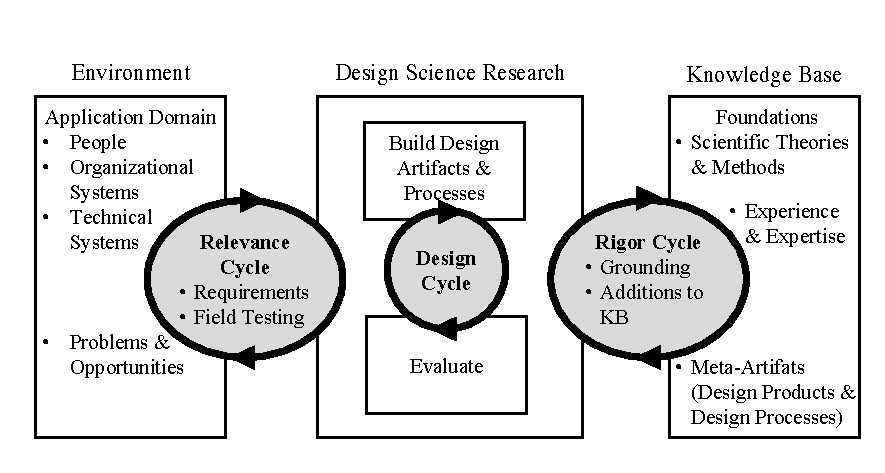
\includegraphics[width=.8\textwidth]{figures/dsr.pdf}
	} \\
\parbox{0.8\textwidth}{\quelle{\citep[\p{16}]{Hevner2010}}}
\end{figure}


\Fig \ref{fig:dsr} shows three research cycles, that should be identifiable in every \acrshort{DSR} project \citep{Hevner2010}. The environment is origin of the wish to design an artifact that solves a particular problem. In this thesis it is the absence of a process model that has referential character in the domain of \acrshort{BPO} providers in \acrshort{CRM}. The contextual environment of the partnering  \acrshort{BPO} provider is used to define requirements, which are transferred via the relevance cycle to the \acrshort{DSR} component. Its inherent design cycle brings together the building of the artifact and its evaluation. An (IT)-artifact can be a model \citep{Hevner2010} like the reference model at hand. Evaluation of the design with help of the relevance cycle ensures that the problem is addressed in a meaningful way. The design itself is connected to the knowledge base via the rigor cycle. It draws from vast knowledge in form of scientific theories or experience and expertise. It bases the design of the artifact on existing knowledge. By using proven methods and structures of reference modeling, a solid foundation is chosen. The application and transfer into the domain is supported by data from literature, as well as by qualitative research in form of interviews with experts. These two data sources are mentioned in the relevant literature \citep[\p{247}]{thomas2006mang}. The separation from routine design implies that a thorough examination is necessary in the design process to ensure the universal applicability of the reference model artifact. 

This work applies the six step method for \acrshort{DSR} proposed by \citep{Hevner2004,Peffers2007}, that consists of: identify problem (1); define solution objectives (2); design and development (3); demonstration (4); evaluation (5); and communication (6). 




%%%%%%%%%%

%
%	\begin{tikzpicture}
%	[node distance=.5cm,
%	start chain=going below,]
%	
%	\node[punktchain, join=by {-}] (investeringer)      {Investeringsteori};
%	\node[punktchain, join=by {-}] (perfekt) {Det perfekte kapitalmarked};
%	\node[punktchain, join=by {-}, ] (emperi) {Emperi};
%	\node (asym) [punktchain ]  {Asymmetrisk information};
%	\begin{scope}[start branch=venstre,
%	%We need to redefine the join-style to have the -> turn out right
%	every join/.style={-, thick, shorten <=1pt}, ]
%	\node[punktchain, on chain=going left, join=by {-}]
%	(risiko) {Risiko og gamble};
%	\end{scope}
%	\begin{scope}[start branch=hoejre,]
%	\node (finans) [punktchain, on chain=going right] {Det finansielle system};
%	\end{scope}
%	\node[punktchain, join=by {-},] (disk) {Det imperfekte finansielle marked};
%	\node[punktchain, join=by {-},] (makro) {Investeringsmssige konsekvenser};
%		\node[punktchain, draw=pink] (aux1) { };
%	\node[punktchain, below right=0.6cm and -1.975cm of makro] (konk) {Konklusion};
%	\node[punktchain,  left = of konk,] (konk2) {Konklusi2on};
%		\node[punktchain, below= of aux1 ] (m1) {m1};
%	% Now that we have finished the main figure let us add some "after-drawings"
%	%% First, let us connect (finans) with (disk). We want it to have
%	%% square corners.
%	\draw[|-,-|,-, thick,] (finans.south) |-+(0,-1em)-| (disk.north);
%	\draw[|-,-|,-, thick,] (emperi.south) |-+(0,-1em)-| (risiko.north);
%	\draw[|-,-|,-, thick,] (emperi.south) |-+(0,-1em)-| (asym.north);
%
%\draw[|-,-|,-, thick,] (makro.south) |-+(0,-0.7em)-| (konk.north);
%\draw[|-,-|,-, thick,] (makro.south) |-+(0,-0.7em)-| (konk2.north);
%
%\draw[|-,-|,-, thick,] (konk.south) |-+(0,-0.7em)-| (m1.north);
%\draw[|-,-|,-, thick,] (konk2.south) |-+(0,-0.7em)-| (m1.north);
%
%	% Now, let us add some braches. 
%
%	\draw[tuborg, decoration={brace}] let \p1=(perfekt.north), \p2=(emperi.south) in
%	($(2.5, \y1)$) -- ($(2.5, \y2)$) node[tubnode] {Problemfelt};
%	\end{tikzpicture}
%		
		
		
	
	%%%%%%%%%%
\section{Empirical Research}
	%%%%%%%%%%
	As stated in the epistemological positioning, a Kantianistic view with cognition from intellect and experience is taken. While the cognition from intellect is of special importance in design of the artifact, the transfer of knowledge from domain experts motivates the cognition from experience in evaluation and requirements specification. 
	%wegkopiert nach vorne
	
	The communication with the research partner was key for gaining insights into the domain. As automated process modeling approaches, like process mining, are not possible due to a lack of suitable data, manual techniques are used. These require a data basis, which builds on the school of empiricism. Qualitative research techniques in form of workshops, document analysis and interviews are used in the research project. 
	
	A plan for the selection of interview candidates was developed in collaboration with the research partner to ensure coverage of the application domain, which is a form of theoretical sampling\footnote{For more information about sampling in qualitative studies see \citep{coyne1997sampling}.}. In a top-down approach managers from core processes in the organization were interviewed face-to-face or by call. For this thesis, interviews with nine domain experts were conducted, transcribed and analyzed. Each interview lasted for \apprx 40 minutes. Additional presentations and documents were provided by the interviewees and served as an additional source of information. Since the thesis is part of an ongoing research project, other data sources that were not directly connected to the thesis are used like the outcomes of a process modeling workshop and notes from previous meetings, where no transcription is available. The process modeling workshop was conducted over two days and included four practitioners and four researchers. 
	
	Analysis of data started before all interviews were conducted, as coverage of fields of interest was necessary on the required detail level. 
	
%interviews
%data, --> ECIS paper draft. 
% analysis of papers?
	
	
